\begin{figure}
  \begin{subfigure}{.45\linewidth}
    \centering
    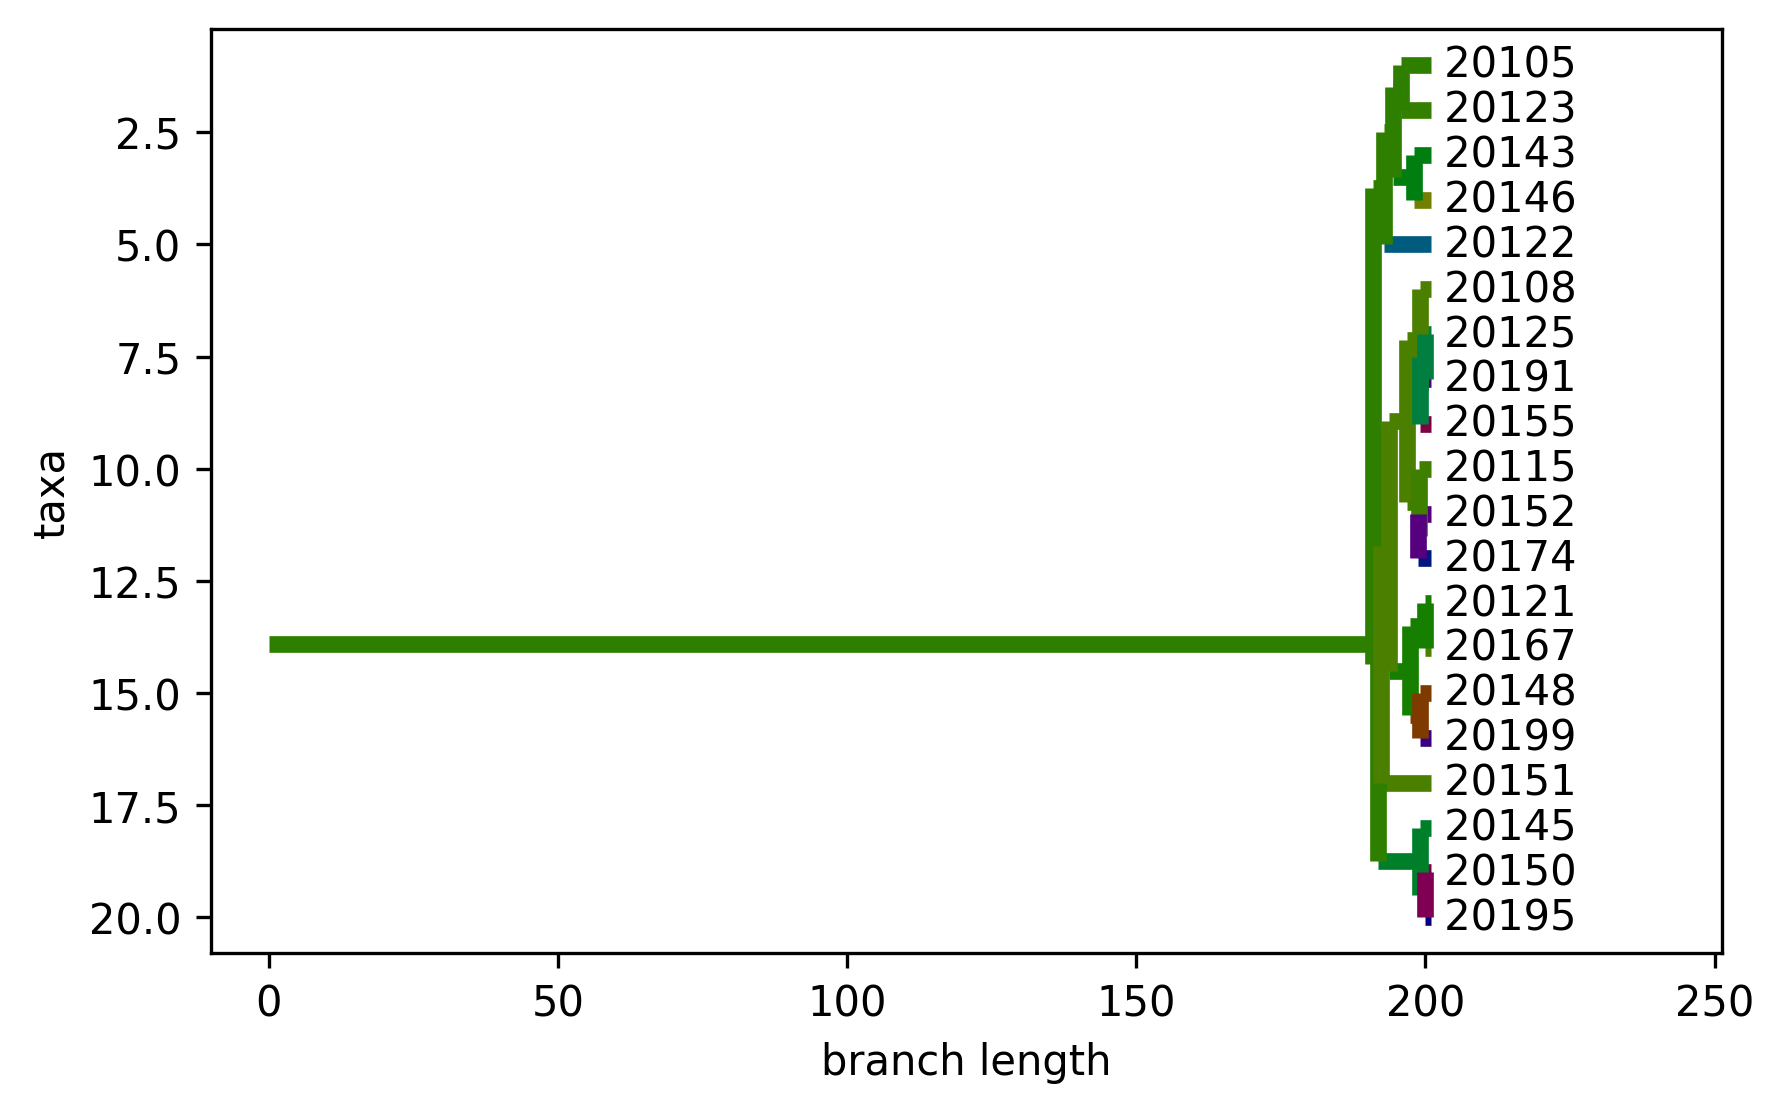
\includegraphics[width=1.05\linewidth]{notebooks/notebooks/teeplots/max_leaves=20+notebook=species-inference+replicate=0+treatment=bag+type=distilled-reference+viz=draw-biopython-tree+ext=}
    \caption{Bag reference}
    \label{fig:species-example-replicates:bag-reference}
  \end{subfigure}
  \,
  \begin{subfigure}{.45\linewidth}
    \centering
    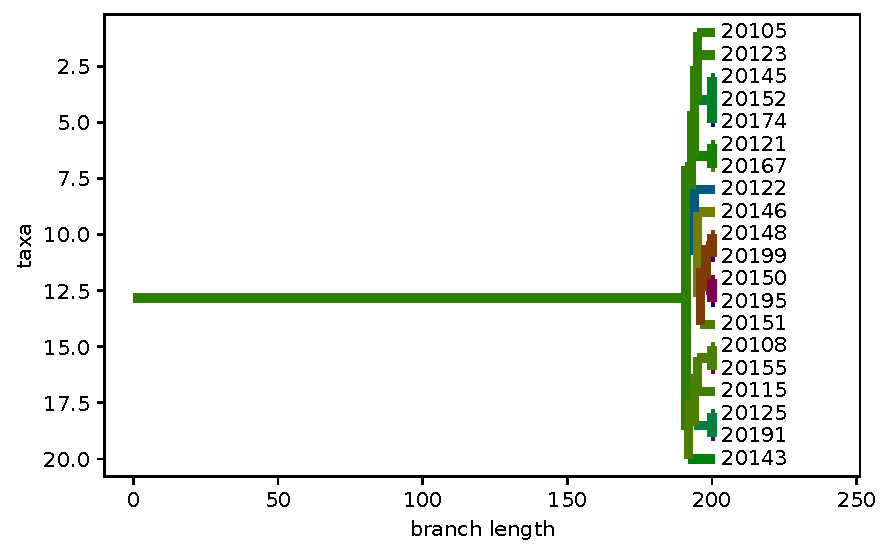
\includegraphics[width=1.05\linewidth]{notebooks/notebooks/teeplots/max_leaves=20+notebook=species-inference+replicate=0+treatment=bag+type=reconstruction+viz=draw-biopython-tree+ext=}
    \caption{Bag reconstruction}
    \label{fig:species-example-replicates:bag-reconstruction}
  \end{subfigure}

  \begin{subfigure}{.45\linewidth}
    \centering
    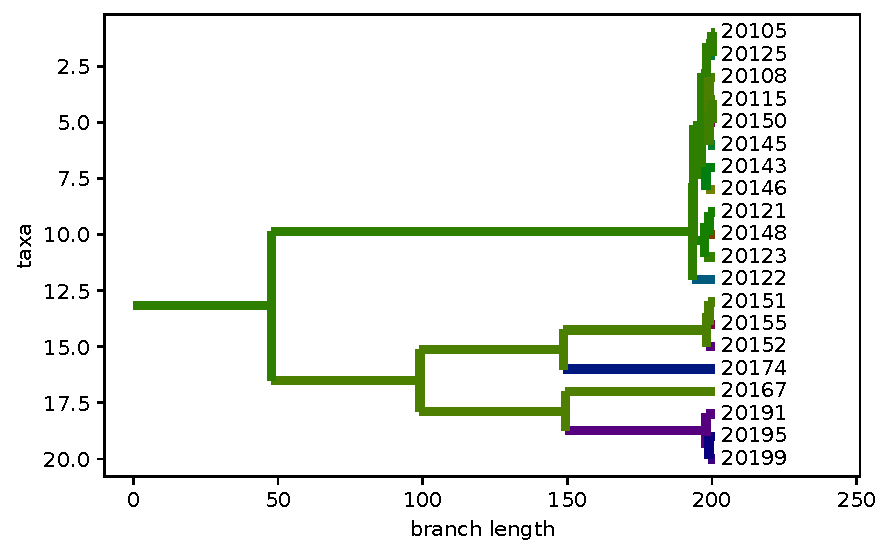
\includegraphics[width=1.05\linewidth]{notebooks/notebooks/teeplots/max_leaves=20+notebook=species-inference+replicate=0+treatment=allopatry+type=distilled-reference+viz=draw-biopython-tree+ext=}
    \caption{Allopatry reference}
    \label{fig:species-example-replicates:allopatry-reference}
  \end{subfigure}
  \,
  \begin{subfigure}{.45\linewidth}
    \centering
    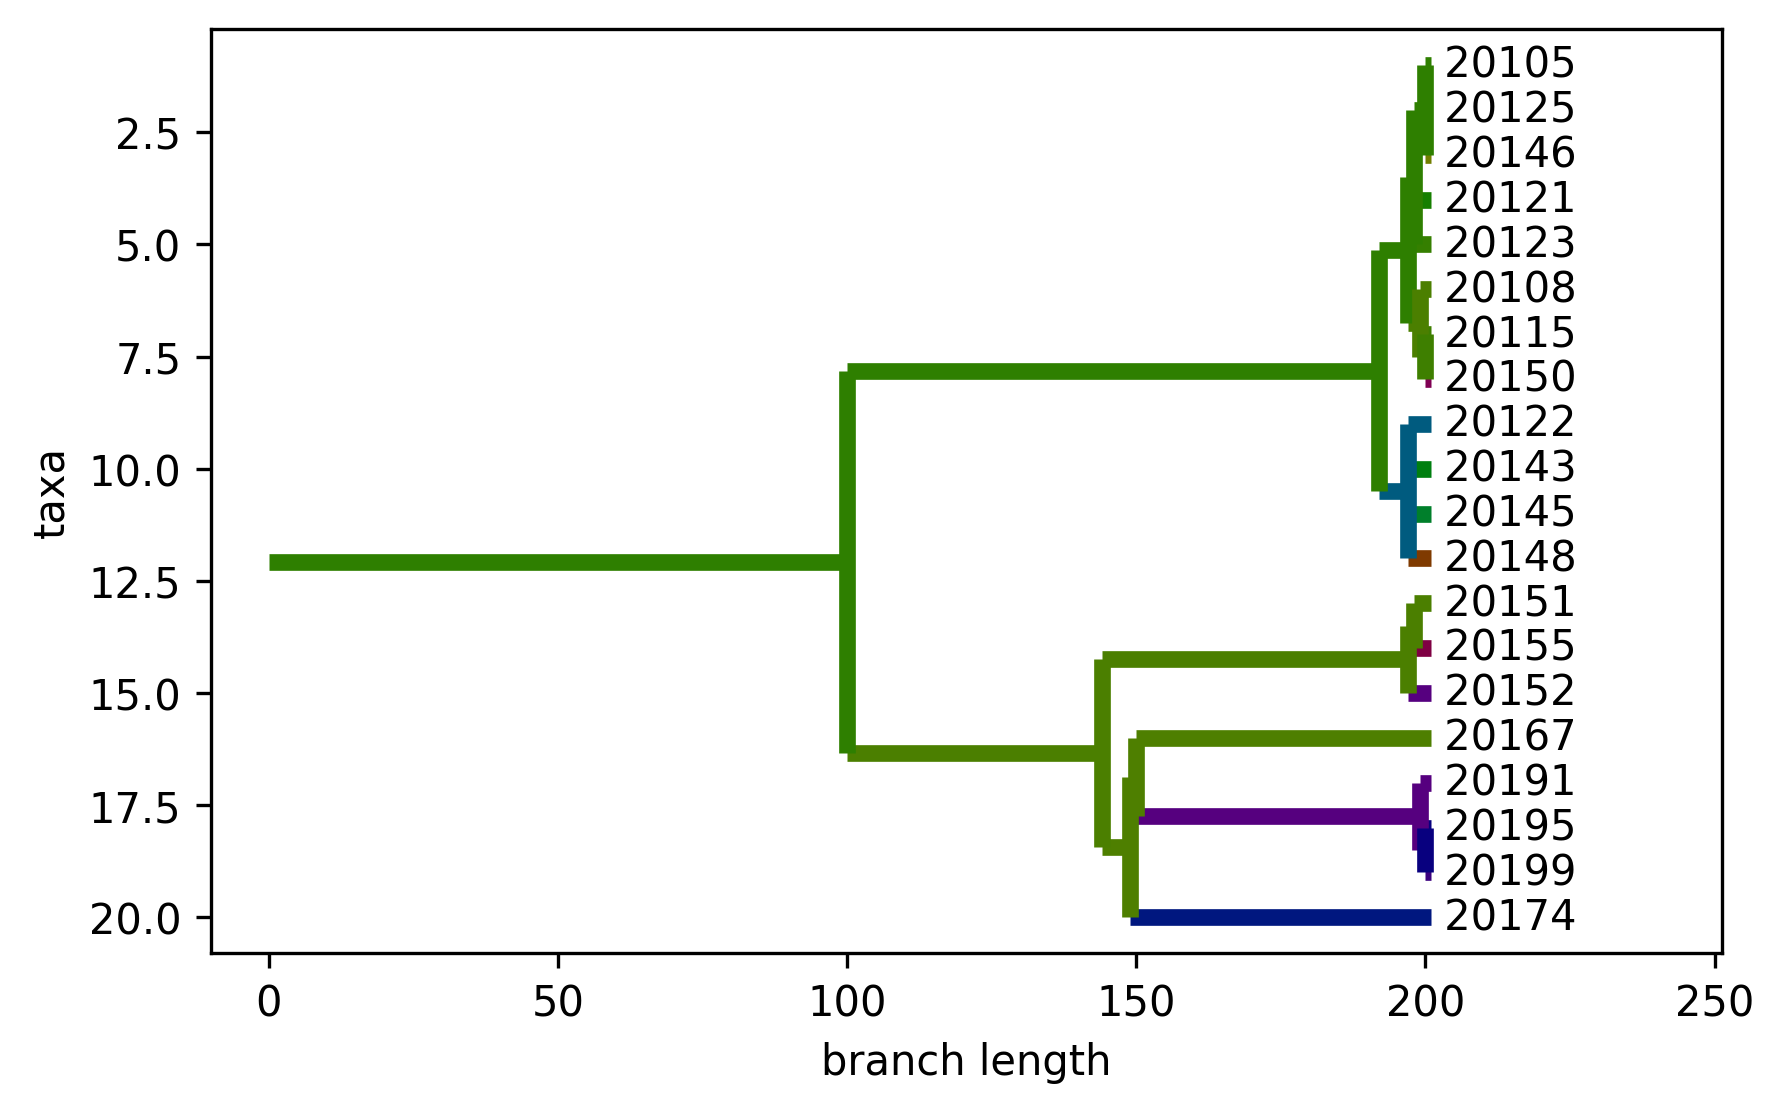
\includegraphics[width=1.05\linewidth]{notebooks/notebooks/teeplots/max_leaves=20+notebook=species-inference+replicate=0+treatment=allopatry+type=reconstruction+viz=draw-biopython-tree+ext=}
    \caption{Allopatry reconstruction}
    \label{fig:species-example-replicates:allopatry-reconstruction}
  \end{subfigure}

  \begin{subfigure}{.45\linewidth}
    \centering
    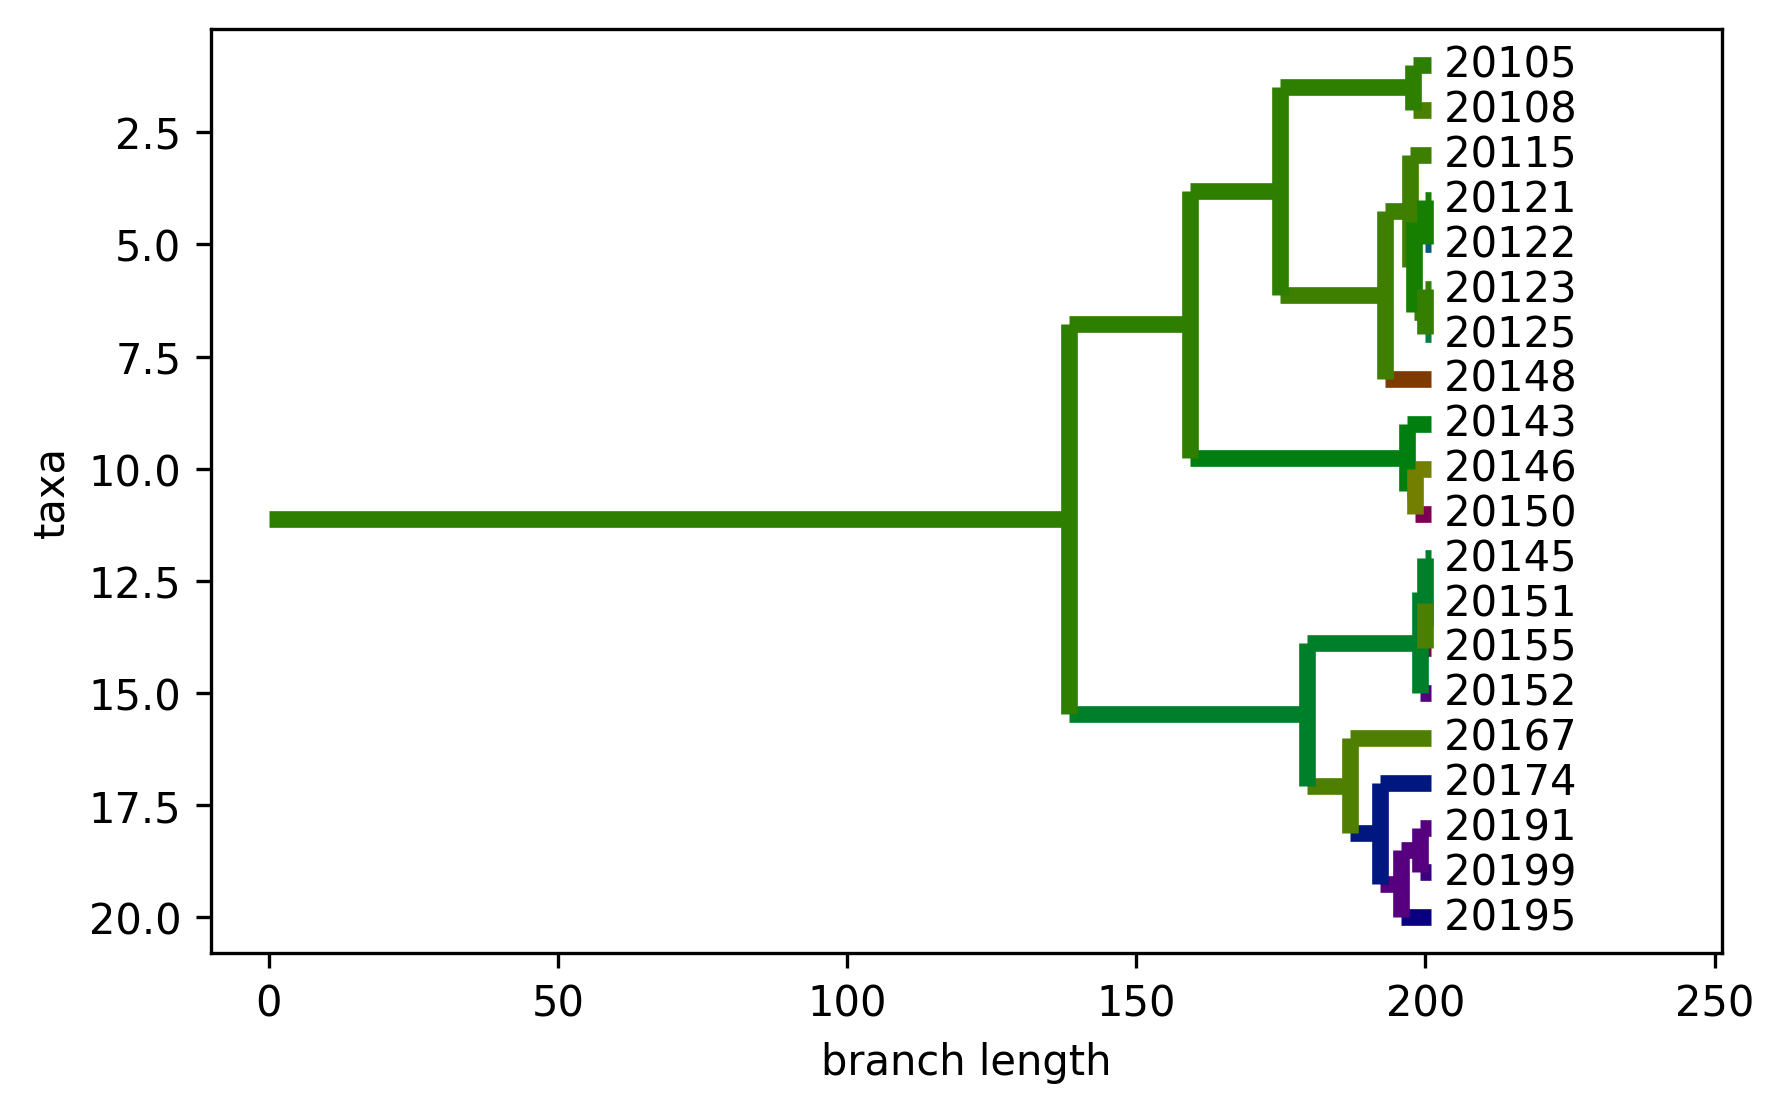
\includegraphics[width=1.05\linewidth]{notebooks/notebooks/teeplots/max_leaves=20+notebook=species-inference+replicate=0+treatment=ring+type=distilled-reference+viz=draw-biopython-tree+ext=}
    \caption{Ring reference}
    \label{fig:species-example-replicates:ring-reference}
  \end{subfigure}
  \,
  \begin{subfigure}{.45\linewidth}
    \centering
    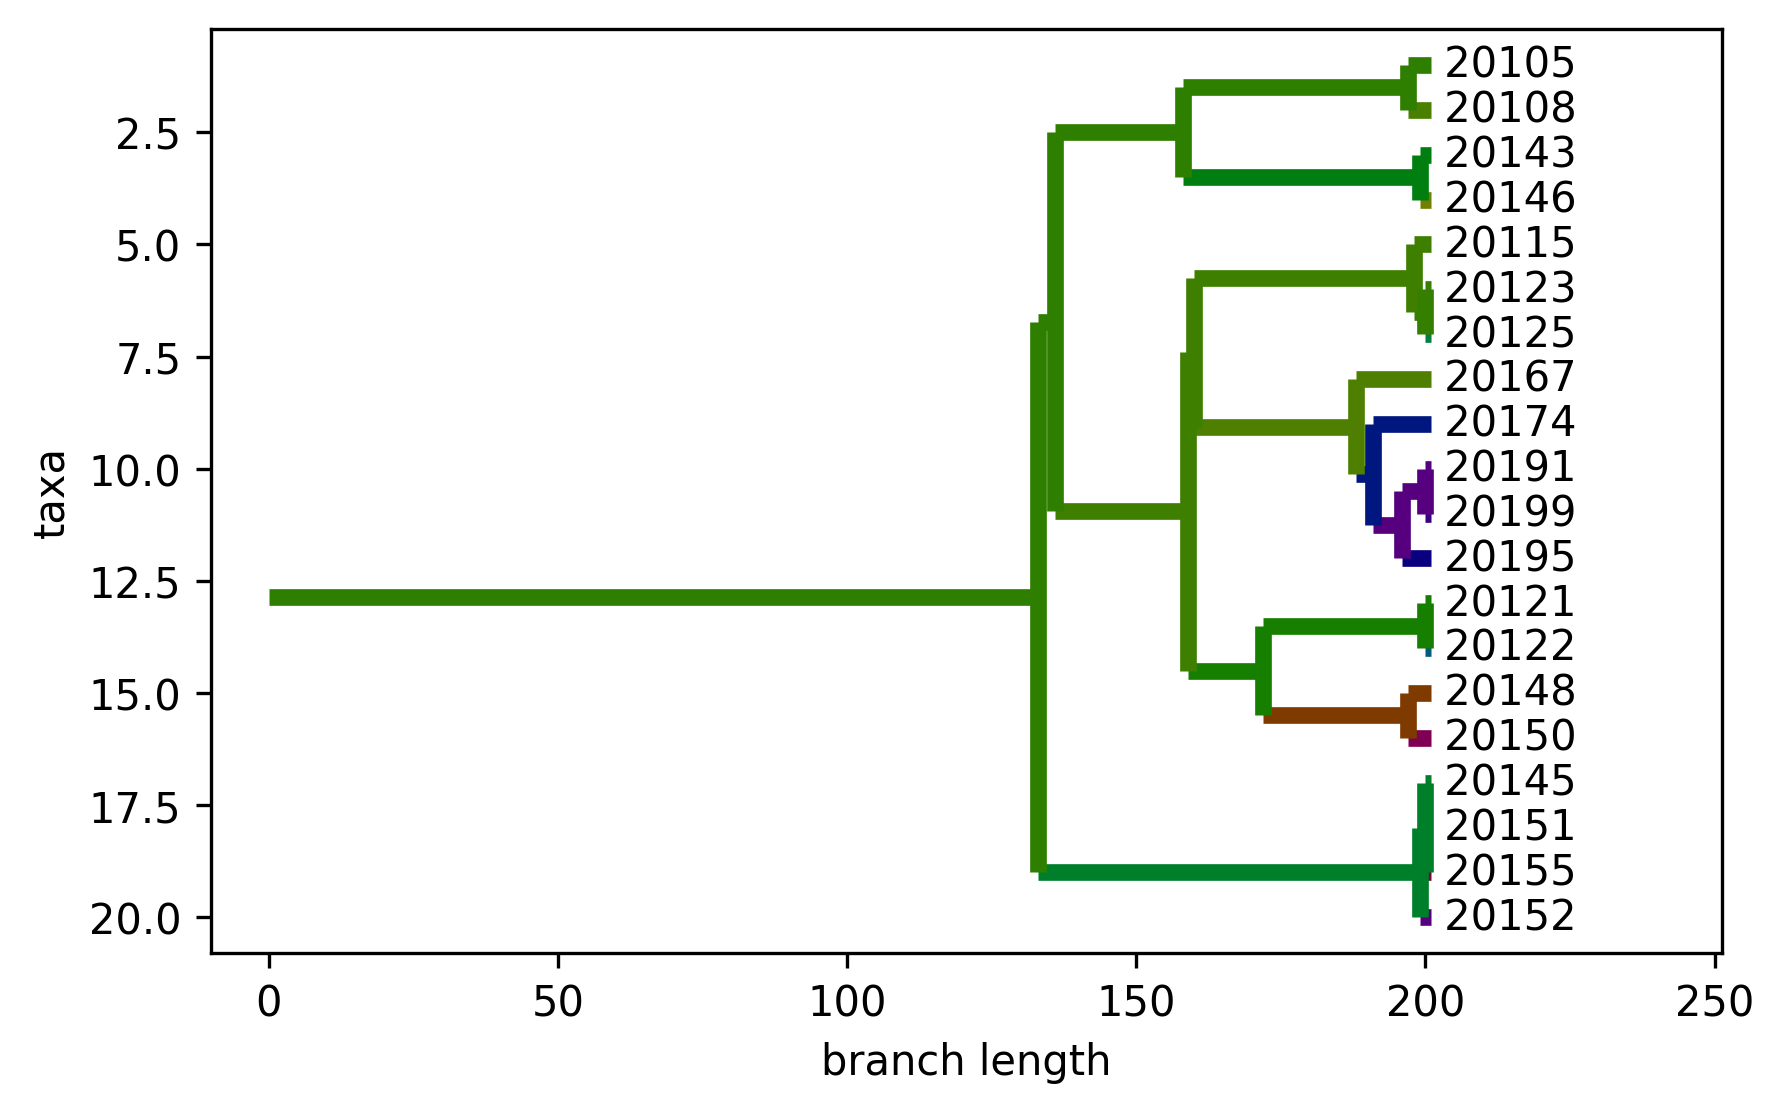
\includegraphics[width=1.05\linewidth]{notebooks/notebooks/teeplots/max_leaves=20+notebook=species-inference+replicate=0+treatment=ring+type=reconstruction+viz=draw-biopython-tree+ext=}
    \caption{Ring reconstruction}
    \label{fig:species-example-replicates:ring-reconstruction}
  \end{subfigure}
  \caption{Comparison of reference phylogenies (top) and reconstructed phylogenies (bottom) for example replicates of each experimental treatment: bag (well-mixed), allopatry (population split at generation 100 with a secondary split on one branch at generation 150), and ring (ten island subpopulations with some migration).
  Phlogenies are downsampled from 100 to 20 tips for legibility.
  Extant organism ID's are annotated on tips.
  Taxon color coding is consistent between reference and reconstruction to facilitate comparison.
  Branch length on $x$ axis given in generations.
  }
  \label{fig:species-example-replicates}

\end{figure}
%
% notebooks/notebooks/teeplots/max_leaves=20+notebook=species-inference+replicate=0+treatment=allopatry+type=distilled-reference+viz=draw-biopython-tree+ext=.pdf
%
% notebooks/notebooks/teeplots/max_leaves=20+notebook=species-inference+replicate=0+treatment=allopatry+type=reconstruction+viz=draw-biopython-tree+ext=.pdf
%
% notebooks/notebooks/teeplots/max_leaves=20+notebook=species-inference+replicate=0+treatment=bag+type=distilled-reference+viz=draw-biopython-tree+ext=.pdf
%
% notebooks/notebooks/teeplots/max_leaves=20+notebook=species-inference+replicate=0+treatment=bag+type=reconstruction+viz=draw-biopython-tree+ext=.pdf
%
% notebooks/notebooks/teeplots/max_leaves=20+notebook=species-inference+replicate=0+treatment=ring+type=distilled-reference+viz=draw-biopython-tree+ext=.pdf
%
% notebooks/notebooks/teeplots/max_leaves=20+notebook=species-inference+replicate=0+treatment=ring+type=reconstruction+viz=draw-biopython-tree+ext=.pdf
